\documentclass{article}

\usepackage{fancyhdr}
\usepackage{extramarks}
\usepackage{amsmath}
\usepackage{amsthm}
\usepackage{amsfonts}
\usepackage{tikz}
\usepackage[plain]{algorithm}
\usepackage{algpseudocode}
\usepackage[utf8]{inputenc}
\usepackage[T1]{fontenc}
\usepackage{natbib}
\usepackage{caption}
\usepackage{subcaption}
\usepackage{listings}

\usetikzlibrary{automata,positioning}

%
% Basic Document Settings
%

\topmargin=-0.45in
\evensidemargin=0in
\oddsidemargin=0in
\textwidth=6.5in
\textheight=9.0in
\headsep=0.25in

\linespread{1.1}

\pagestyle{fancy}
%\lhead{\hmwkAuthorName}
%\chead{\hmwkClass\ (\hmwkClassInstructor\ \hmwkClassTime): \hmwkTitle}
\lhead{\hmwkClass: \hmwkTitle}
\rhead{\hmwkAuthorName}
\lfoot{\lastxmark}
\cfoot{\thepage}

\renewcommand\headrulewidth{0.4pt}
\renewcommand\footrulewidth{0.4pt}

\setlength\parindent{0pt}
\setlength{\parskip}{1em}

%
% Create Problem Sections
%

\newcommand{\enterProblemHeader}[1]{
    \nobreak\extramarks{}{Problem \arabic{#1} continued on next page\ldots}\nobreak{}
    \nobreak\extramarks{Problem \arabic{#1} (continued)}{Problem \arabic{#1} continued on next page\ldots}\nobreak{}
}

\newcommand{\exitProblemHeader}[1]{
    \nobreak\extramarks{Problem \arabic{#1} (continued)}{Problem \arabic{#1} continued on next page\ldots}\nobreak{}
    \stepcounter{#1}
    \nobreak\extramarks{Problem \arabic{#1}}{}\nobreak{}
}

\setcounter{secnumdepth}{3}
\newcounter{partCounter}
\newcounter{homeworkProblemCounter}
\setcounter{homeworkProblemCounter}{1}
%\nobreak\extramarks{Problem \arabic{homeworkProblemCounter}}{}\nobreak{}

%
% Homework Problem Environment
%
% This environment takes an optional argument. When given, it will adjust the
% problem counter. This is useful for when the problems given for your
% assignment aren't sequential. See the last 3 problems of this template for an
% example.
%
\newenvironment{homeworkProblem}[1][-1]{
    \ifnum#1>0
        \setcounter{homeworkProblemCounter}{#1}
    \fi
    \section{Problem \arabic{homeworkProblemCounter}}
    \setcounter{partCounter}{1}
    \enterProblemHeader{homeworkProblemCounter}
}{
    \exitProblemHeader{homeworkProblemCounter}
}

%
% Homework Details
%   - Title
%   - Due date
%   - Class
%   - Section/Time
%   - Instructor
%   - Author
%

\newcommand{\hmwkTitle}{Rapport Final}
\newcommand{\hmwkDueDate}{30 avril, 2017}
\newcommand{\hmwkClass}{MTH8408}
\newcommand{\hmwkClassTime}{}
\newcommand{\hmwkClassInstructor}{Professeur Dominique Orban}
\newcommand{\hmwkAuthorName}{André Phu-Van Nguyen, 1525972}
\renewcommand{\refname}{Références}

%
% Title Page
%

\title{
    \vspace{2in}
    \textmd{\textbf{\hmwkClass:\ \hmwkTitle}}\\
    \normalsize\vspace{0.1in}\small{Remis\ pour\ le\ \hmwkDueDate\ }\\
    \vspace{0.1in}\large{\textit{\hmwkClassInstructor\ \hmwkClassTime}}
    \vspace{3in}
}

\author{\textbf{\hmwkAuthorName}}
\date{}

\renewcommand{\part}[1]{\textbf{\large Part \Alph{partCounter}}\stepcounter{partCounter}\\}

%
% Various Helper Commands
%

% Useful for algorithms
\newcommand{\alg}[1]{\textsc{\bfseries \footnotesize #1}}

% For derivatives
\newcommand{\deriv}[1]{\frac{\mathrm{d}}{\mathrm{d}x} (#1)}

% For partial derivatives
\newcommand{\pderiv}[2]{\frac{\partial}{\partial #1} (#2)}

% Integral dx
\newcommand{\dx}{\mathrm{d}x}

% Alias for the Solution section header
\newcommand{\solution}{\textbf{\large Solution}}
\newcommand{\norm}[1]{\left\lVert#1\right\rVert}

% Probability commands: Expectation, Variance, Covariance, Bias
\newcommand{\E}{\mathrm{E}}
\newcommand{\Var}{\mathrm{Var}}
\newcommand{\Cov}{\mathrm{Cov}}
\newcommand{\Bias}{\mathrm{Bias}}

\begin{document}

\maketitle

\pagebreak

\section{Rappel de la problématique}

Ce projet consiste en l'étude et l'implémentation de l'article \textit{Minimum Snap Trajectory Generation and Control for Quadrotors} par Daniel Mellinger et Vijay Kumar \cite{Mellinger2011} qui propose un contrôleur et un générateur de trajectoires pour un véhicule aérien multirotor. Plus précisément, nous faisont une implémentation seulement de la partie génération de trajectoire par une méthode d'optimisation numérique.

Lors du suivi d'une trajectoire, une solution triviale est souvent utilisée qui consiste en l'interpolation en ligne droite entre chaque point de cheminement ou \textit{waypoint} (Mellinger utilise plutôt l'apellation \textit{keyframe}). Ceci est inneficace car la courbure infinie à chaque waypoint oblige le quadricoptère à s'arrêter avant de passer au prochain waypoint. Mellinger propose donc de modéliser une trajectoire optimale par un polynôme défini par parties entièrement lisse à travers les différents waypoints tout en satisfaisant des contraintes sur les vitesses et accélérations possibles du véhicule. Ce problème est résolu en le reécrivant en problème d'optimisation quadratique.

Tout dabord Mellinger démontre que la dynamique d'un quadricoptère a la propriété dêtre différentiellement plat. C'est-à-dire que les états et les entrées peuvent être exprimées par les sorties du système et leurs dérivées. Nous avons donc le vecteur de sorties plates
$$\sigma = [x, y, z, \psi]^T$$
où $r = [x, y, z]^T$ est la position du centre de masse dans le système de coordonnées du monde et $\psi$ l'angle de lacet. Rappelons nous que dans un repère main droite centré sur un corps rigide, l'axe $x$ pointe vers l'avant, $y$ vers la gauche et $z$ vers le haut. Les angles de rotation autour de ces axes sont le roulis (\textit{roll}), tangage (\textit{pitch}) et lacet (\textit{yaw}) respectivement. À fin de garder le projet simple, nous ne considérons pas les angles de roulis et de tangage dans le problème mais nous savons qu'il est possible de le faire pour exécuter des manoeuvres accrobatiques tel que voler à travers une fenêtre inclinée.

\begin{figure}[h]
	\centering
	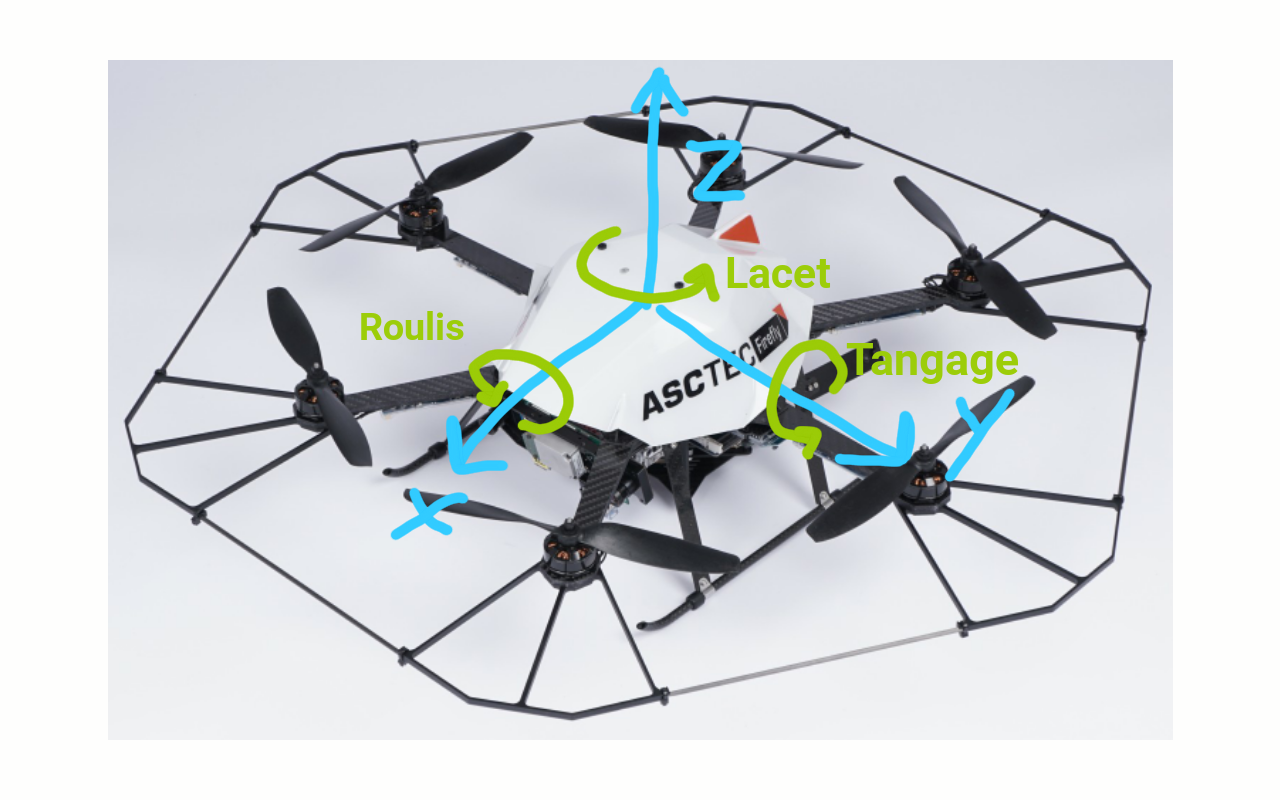
\includegraphics[width=0.5\textwidth]{fig/firefly.png}
	\caption{Systèmes de coordonnées d'un hexacoptère. L'angle de lacet est la rotation du véhicule autour de son axe Z, c'est-à-dire quand le véhicule tourne sur lui même.}
\end{figure}

Une trajectoire est définie comme était une courbe lisse dans l'espace des sorties plates:
$$ \sigma(t) : [t_0, t_m] \rightarrow \mathbb{R}^3 \times SO(2)$$
où $t_0$ et $t_m$ sont les temps de début et de fin de la trajectoire, $m$ correspond au nombre d'intervales de temps entre chaque waypoint et $SO(2)$ est le groupe spécial orthogonal. En pratique, une trajectoire est plutôt décrite par un polynôme défini par parties:
\begin{align}\label{eq:polynomial}
\sigma_T(t) =
\left\{
	\begin{array}{ll}
		\sum_{i=0}^n \sigma_{Ti1} t^i  & t_0 \leq t < t_1 \\
		\sum_{i=0}^n \sigma_{Ti2} t^i  & t_1 \leq t < t_2 \\
		... \\
		\sum_{i=0}^n \sigma_{Tim} t^i  & t_{m-1} \leq t < t_m \\
	\end{array}
\right.
\end{align}
où $n$ est l'ordre du polynôme et $m$ est encore le nombre d'intervales de temps.

Étant donné que l'on veut optimiser la dérivée d'ordre $k_r = 4$ (le \textit{snap}) de la position au carré et la dérivée d'ordre $k_\psi = 2$ (accélération angulaire) de langle de lacet $\psi$ au carré, nous avons le problème d'optimisation:
\begin{align}\label{eq:opt}
\text{min} \int_{t_0}^{t_m} \mu_r \norm{\frac{d^4 \boldsymbol{r}_T}{dt^4}}^2 + \mu_\psi {\ddot{\psi}_T}^2 dt
\end{align}\begin{align*}
	\begin{array}{lll}
%		\text{sous contraintes} & \sigma_T(t_i) = \sigma_i & i = 0, \ldots, m\\
		\text{sous contraintes} & \boldsymbol{r}_T(t_i) = \boldsymbol{r}_i & i = 0, \ldots, m\\
		& \psi_T(ti)=\psi_i & i = 0, \ldots, m\\
		& \frac{d^p x_T}{dt^p}|_{t=t_j} = 0\ \text{ou libre,} & j = 0, m; p = 1, 2, 3, 4\\
		& \frac{d^p y_T}{dt^p}|_{t=t_j} = 0\ \text{ou libre,} & j = 0, m; p = 1, 2, 3, 4\\
		& \frac{d^p z_T}{dt^p}|_{t=t_j} = 0\ \text{ou libre,} & j = 0, m; p = 1, 2, 3, 4\\
		& \frac{d^p \psi_T}{dt^p}|_{t=t_j} = 0\ \text{ou libre,} & j = 0, m; p = 1, 2\\
	\end{array}
\end{align*}

où $\boldsymbol{r}_T = [x_T, y_T, z_T]^T$ et $r_i = [x_i, y_i, z_i]$.

\section{Structure du problème d'optimisation}

\subsection{Problème d'optimisation quadratique}

Puisque l'article de Mellinger comporte très peu de détails et ne discute de la manière de poser le problème que vaguement, nous avons été obligé de faire le développement des équations à la main et au final nous avons aussi été obligé de consulter d'autres articles (Bry et Richter) citant celui de Mellinger pour mieux comprendre comment faire. Le dévelppement mathématique suivant est donc un mélange de notre propre travail et de ce qui est écrit dans \cite{Richter2016, bry2012control}.

Considérons le problème en une dimension $p$, où $p = x$, $y$ ou $z$. Nous pouvons reformuler le problème en tant que problème d'optimisation quadratique en réécrivant les coefficients des polynômes en un vecteur $c$ de dimension $4m \times 1$, où $m$ est le nombre de waypoints en excluant les conditions initiales. Nous obtenons la forme standard avec contraintes d'égalité linéaires:
\begin{equation}\label{eq:opt_quad}
\begin{aligned}
& \underset{c}{\text{min}}
& & c^THc+f^Tc \\
& \text{s. c.}
& & Ac = b
\end{aligned}
\end{equation}
Par exemple si $n=6$ nous avons un polynôme $p$ représentant un segment de trajectoire:
\begin{align}\label{eq:polynomial}
	p = c_6 t^6 + c_5 t^5 + c_4 t^4 + c_3 t^3 + c_2 t^2 + c_1 t + c_0
\end{align}

Donc le vecteur $c = [c_6, c_5, c_4, c_3, c_3, c_2, c_1, c_0]^T$ est le vecteur des coefficients des polynômes. Nous notons aussi que la partie linéaire $f^Tc$ est nulle.

\subsubsection{Construction de la matrice hessienne}

Pour un axe de déplacement $p$ et un waypoint $j$, Richter et Bry \cite{Richter2016, bry2012control} indiquent que le processus de construction de la matrice $H$ peut être automatisé par la formule suivante:
\begin{align}
H_{pj} =\left\{
  \begin{array}{ll}
    2 \Big( \prod_{m = 0}^{r-1} (i-m)(l-m)\Big) \frac{\tau^{i+l-2r+1}}{i+l-2r+1}: & i \geq r \text{ ou } l \geq r \\
    0 : & \text{autrement}
  \end{array}
  \right.
\end{align}
où $i$ et $l$ sont les index de rangée et de colonne et $\tau$ est la durée du segment de trajectoire.\footnote{Il faut faire une rotation de $180$ degrés sur la matrice résultante pour avoir les puissances plus hautes dans les index plus bas.} Concrètement, cela donne lieu à une matrice de la forme suivante:
\begin{align}\label{eq:hessienne_p}
H_{pj} =
\begin{bmatrix}
    360^2 \frac{1}{5} t^5 \Big|_{t_j}^{t_{j+1}}
    		& 2 \cdot 360 \cdot 120 \frac{1}{4} t^4\Big|_{t_j}^{t_{j+1}}
    		& 2 \cdot 360 \cdot 24 \frac{1}{3} t^3\Big|_{t_j}^{t_{j+1}}
    		& 0
    		& 0
    		& 0
	    	& 0 \\
    2 \cdot 360 \cdot 120 \frac{1}{4} t^4\Big|_{t_j}^{t_{j+1}}
    		& 120^2 \frac{1}{3} t^3\Big|_{t_j}^{t_{j+1}}
    		& 2 \cdot 120 \cdot 24 \frac{1}{2}t^2 \Big|_{t_j}^{t_{j+1}} & 0 & 0 & 0 & 0\\
	2 \cdot 360 \cdot 24 \frac{1}{3} t^3\Big|_{t_j}^{t_{j+1}}
		& 2 \cdot 120 \cdot 24 \frac{1}{2}t^2 \Big|_{t_j}^{t_{j+1}}
		& 24^2 t\Big|_{t_j}^{t_{j+1}} & 0 & 0 & 0 & 0 \\
    0 & 0 & 0 & 0 & 0 & 0 & 0 \\
    0 & 0 & 0 & 0 & 0 & 0 & 0 \\
    0 & 0 & 0 & 0 & 0 & 0 & 0 \\
    0 & 0 & 0 & 0 & 0 & 0 & 0 \\
\end{bmatrix}
\end{align}
où $t_j$ et $t_{j+1}$ sont les temps de départ et de fin d'un segment de trajectoire.


La matrice Hessienne finale est construite en concaténant en diagonale les matrices $H_{pj}$ pour chaque waypoint jusqu'à $j=m$ pour former $H$ de (\ref{eq:opt_quad}).

\begin{align}
H_x=
\begin{bmatrix}
	H_{x1} \\
	&	H_{x2} \\
	&	&		\ddots \\
	&	&		&		H_{xm}
\end{bmatrix}
\end{align}

\subsubsection{Construction des contraintes linéaires}

Dans ce problème nous utilisons les matrices de contraintes d'égalité de deux façons. Premièrement pour imposer la valeur d'une certaine dérivée à un certain moment et deuxièmement pour imposer la continuité entre deux segments de trajectoire.

Dans notre code, nous avons appelé ceci les contraintes de départ et d'arrivée et les contraintes de continuité. Encore une fois, nous suivons la formulation de Bry \cite{bry2012control}(car Mellinger donne peu de détails dans son article) où pour un segment de trajectoire allant du temps $0$ au temps $\tau$ nous pouvons contruire $A$ et $b$ de telle manière que
\begin{align}
A = \begin{bmatrix} A_0 \\ A_\tau \end{bmatrix},\ \ b = \begin{bmatrix} b_0 \\ b_\tau \end{bmatrix}
\end{align}
\begin{align}
A_{0_{rn}} = \left\{
  \begin{array}{ll}
    \prod_{m = 0}^{r-1} (r-m): & r = n \\
    0 : & \text{autrement}
  \end{array}
\right.
\end{align}
\begin{align}
b_{0_r} = P^{(r)}(0)
\end{align}
\begin{align}
A_{\tau_{rn}} = \left\{
  \begin{array}{ll}
    \big(\prod_{m = 0}^{r-1} (n-m) \Big) \tau^{n-r} : & n \geq r \\
    0 : & \text{autrement}
  \end{array}
\right.
\end{align}
\begin{align}
b_{\tau_r} = P^{(r)}(\tau)
\end{align}

Notons que $A_0$ et $A_\tau$ ont $r+1$ rangées (une par dérivée incluant la dérivée 0) et $n$ colonnes (une par coefficient du polynôme). La notation $P^{(r)}(0)$ indique le polynôme dérivé au degré $r$ et évalué au temps $0$. Si jamais la dérivée est sans contrainte, par exemple si nous ne boulons pas imposer la valeur de l'accélération à un certain waypoint, il suffit simplement d'ommettre la ligne correspondante de la matrice $A$.

En appliquant les équations précédentes, nous imposons à chaque waypoint une valeur fixe pour la position, la vitesse, le \textit{jerk} et le \textit{snap}. Tant à l'arrivée qu'au départ de celui ci. Par contre, si jamais l'utilisateur n'impose pas de contraintes sur ces dérivées, il faut tout de même ajouter des contraintes de continuité pour imposer que la valeur calculée (par le processus d'optimisation) pour cette dérivée soit continue au waypoint. Pour ce faire, il suffit de mettre égal les deux polynômes représentant les segments de part et d'autre d'un waypoint. Soit le polynôme dérivé $r$ fois allant au waypoint $j$, $P_{j}^{(r)}$ et le prochain polynôme partant du waypoint $j$, $P_{j+1}^{(r)}$ nous avons la contrainte

\begin{align*}
	P_{j}^{(r)} &= P_{j+1}^{(r)}\\
	-P_{j+1}^{(r)} + P_{j}^{(r)} &= 0
\end{align*}

Par inspection, nous pouvons recouvrir la forme de $A$ finale proposée par Bry \citep{bry2012control}. Prenons la notation $A_0^j$ la matrice de contraintes pour un début de trajectoire au waypoint $j$ et de même pour $A_\tau^j$ la matrice de contraintes pour une fin de trajectoire au waypoint $j$. Nous avons au final:
\begin{align}
A=  \begin{bmatrix}
		A_0^0	& 0	& 0 & 0 & \ldots & 0 & 0 \\
		-A_\tau^0 & A_0^1 & 0 & 0 & \ldots & 0 & 0 \\
		0 &  -A_\tau^1 & A_0^2 & 0 & \ldots & 0 & 0\\
		0 & 0 & -A_\tau^2 & A_0^3 & \ldots &0 &0 \\
		\ldots & \ldots & \ldots & \ldots & \ddots & \ldots & \ldots \\
		0& 0& 0& 0& 0& -A_\tau^{m-1} & A_0^m \\
				0& 0& 0& 0& 0& 0& A_\tau^m
	\end{bmatrix}
\end{align}
\begin{align}
b = \left\{
  \begin{array}{ll}
    \text{Valeur de la dérivée du polynôme $P$ imposée}: & \text{Si imposé} \\
    0 : & \text{autrement}
  \end{array}
\right.
\end{align}

\textbf{Exemple de matrice de contrainte}

Prenons pour exemple la situation où en $x$ nous avons les waypoints $0, 1$ et $2$ et les temps $t = [0, 1, 2]$ nous obtenons:
\setcounter{MaxMatrixCols}{20}
\begin{align*}
A_xc - b_x = \begin{bmatrix}
0 &  0 &  0 &  0 &  0 &  0 &  1 &  0 &  0 &  0 &  0 &  0 &  0 &  0\\
0 &  0 &  0 &  0 &  0 &  1 &  0 &  0 &  0 &  0 &  0 &  0 &  0 &  0\\
0 &  0 &  0 &  0 &  2 &  0 &  0 &  0 &  0 &  0 &  0 &  0 &  0 &  0\\
0 &  0 &  0 &  6 &  0 &  0 &  0 &  0 &  0 &  0 &  0 &  0 &  0 &  0\\
1 &  1 &  1 &  1 &  1 &  1 &  1 &  0 &  0 &  0 &  0 &  0 &  0 &  0\\
0 &  0 &  0 &  0 &  0 &  0 &  0 &  0 &  0 &  0 &  0 &  0 &  0 &  1\\
0 &  0 &  0 &  0 &  0 &  0 &  0 &  1 &  1 &  1 &  1 &  1 &  1 &  1\\
6 &  5 &  4 &  3 &  2 &  1 &  0 &  0 &  0 &  0 &  0 &  0 &  -1 &  0\\
30 &  20 &  12 &  6 &  2 &  0 &  0 &  0 &  0 &  0 &  0 &  -2 &  0 &  0\\
120 &  60 &  24 &  6 &  0 &  0 &  0 &  0 &  0 &  0 &  -6 &  0 &  0 &  0\\
360 &  120 &  24 &  0 &  0 &  0 &  0 &  0 &  0 &  -24 &  0 &  0 &  0 &  0\\
\end{bmatrix}\begin{bmatrix}
c_{16} \\ c_{15} \\ c_{14} \\ c_{13} \\ c_{12} \\ c_{11} \\ c_{10} \\ c_{16} \\ c_{15} \\ c_{14} \\ c_{13} \\ c_{12} \\ c_{11} \\ c_{10}
\end{bmatrix} -  \begin{bmatrix}
0 \\ 0 \\ 0 \\ 0 \\ 1 \\ 1 \\ 2 \\ 0 \\ 0 \\ 0 \\ 0
\end{bmatrix} = 0
\end{align*}

\subsection{Problème d'optimisation des temps de segment}

Mellinger montre que si jamais le temps d'arrivé à chaque segment n'importe pas, il est possible dans un deuxième temps de résoudre un deuxième problème d'optimisation à fin de trouver la meilleur répartition de temps possible entre chaque segment de la trajectoire.

Au lieu de considérer les temps d'arrivés $t_i$ à un waypoint $i$, nous pouvons plutôt considérer le temps de durée d'un segment de trajectoire $T_i = t_i - t_{i-1}$ et $T = [T_0, T_1, ..., T_i]$. Soit $f(T) = f_x(T) +  f_y(T) + f_z(T)$, la somme des valeurs de fonction de coût après la résolution du problème (\ref{eq:opt_x}) dans chaque dimension. Nous résolvons maintenant le problème
\begin{align}\label{eq:time_opt}
\text{min}\ \ \ f(T)
\end{align}\begin{align*}
\begin{array}{lll}
\text{s. c.} & \sum T_i = t_m & i = 1,\ldots,m\\
& T_i \geq 0 &  i = 1,\ldots,m\\
\end{array}
\end{align*}
où $T_i = t_i - t_{i-1}$ sont les temps alloués à chaque segment de la trajectoire. Il est relativement trivial de reécrire le problème sous la forme standard
\begin{align*}
\text{min}\ \ \ f(x)\\
\begin{array}{lll}
\text{s. c.} & Ax = b\\
& \text{lb} \leq x\\
\end{array}
\end{align*}
$A$ est de taille $1 \times m$ avec des $1$ partout $b = t_m$ le temps d'arrivé au dernier waypoint et lb$=0$. 

Par contre, ce qui est un peu moins trivial est la façon de fournir le gradient de $f(T)$ à la fonction d'optimisation. Mellinger le calcule numériquement par l'équation
\begin{align}
	\nabla_{g_i}f = \frac{f(T + hg_i) - f(T)}{h}
\end{align}
où h est une "petite" valeur et le vecteur colonne.\footnote{Mellinger utilse en fait $\frac{-1}{m-2}$ car son $m$ inclut aussi les conditions initiales.} Donc, pour chaque direction du gradient, il faut rerésoudre le problème d'optimisation (\ref{eq:opt}), ce qui explique pourquoi nous devons utiliser cette méthode numérique au lieu d'une méthode plus performante tel que la différentiation automatique.
\begin{align}
g_i = \left\{
  \begin{array}{ll}
    1: & \text{à la position }i  \\
    \frac{-1}{m-1} : & \text{autrement}
  \end{array}
\right.
\end{align}
par exemple, dans le cas où $m=3$ nous aurions
\begin{align*}
	g_1 = \begin{bmatrix} 1\\ -\frac{1}{2} \\-\frac{1}{2} 	\end{bmatrix}\text{, }
	g_2 = \begin{bmatrix} -\frac{1}{2}\\ 1 \\-\frac{1}{2} 	\end{bmatrix}\text{ et }
	g_3 = \begin{bmatrix} -\frac{1}{2} \\-\frac{1}{2}\\ 1 	\end{bmatrix}
\end{align*}
et le gradient final serait
\begin{align*}
\nabla f = \begin{bmatrix}
	\nabla_{g_1}f\\
	\nabla_{g_2}f\\
	\nabla_{g_3}f\\
\end{bmatrix} = \begin{bmatrix}
	 \frac{f(T + hg_1) - f(T)}{h}\\
	 \frac{f(T + hg_2) - f(T)}{h}\\
	 \frac{f(T + hg_3) - f(T)}{h}\\
\end{bmatrix}
\end{align*}

\section{Implémentation}
\subsection{Prototype en Matlab}

Le prototype initial s'est fait au moyen de Matlab et des solveurs \texttt{quadprog} pour la génération de trajectoire et \texttt{fmincon} pour l'optimisation des temps de trajectoire. Pour commencer nous avons reproduit les résultats de Mellinger en faisait une trajectoire simple à travers les points $(0,0)$, $(1,0)$, $(1,2)$ et $(0,2)$ avec une allocation de temps égale à chaque segment de trajectoire et aucune contrainte sur les derivées, outre celles de continuité.

\begin{figure}[h]
\centering
\begin{subfigure}{.4\textwidth}
  \centering
  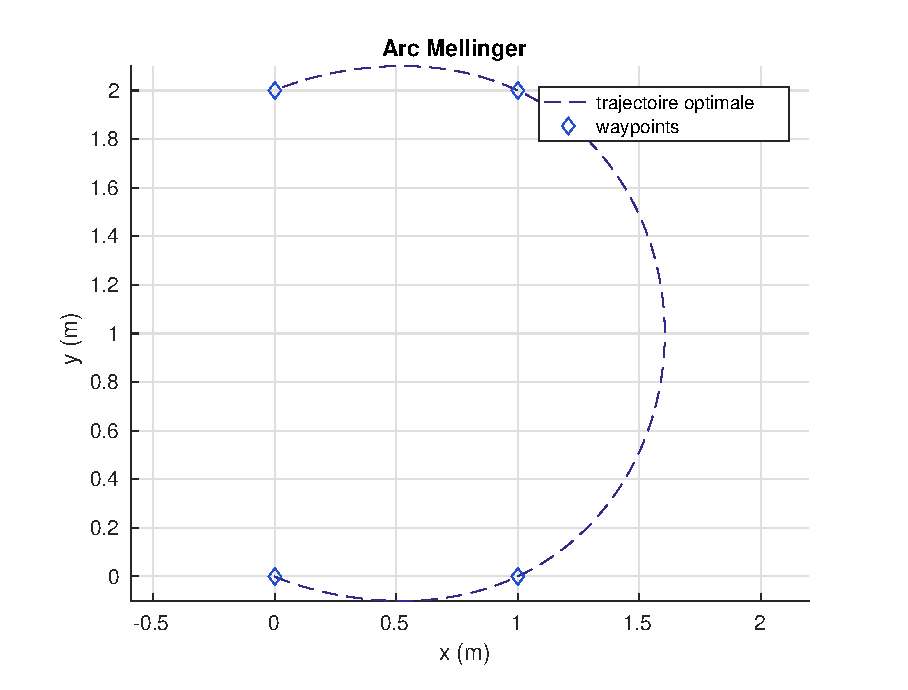
\includegraphics[width=\textwidth]{fig/arc_mellinger}
  \caption{Notre résultat}
\end{subfigure}%
\begin{subfigure}{.4\textwidth}
  \centering
  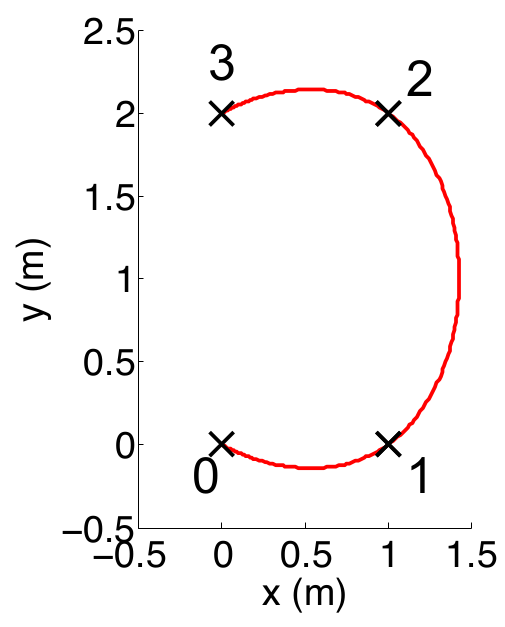
\includegraphics[width=0.6\textwidth]{fig/arc_mellinger_orig.png}
  \caption{Résultat de Mellinger \cite{Mellinger2011}}
  \label{fig:sub2}
\end{subfigure}
\caption{Comparaison de résultats}
\label{fig:comparaison}
\end{figure}

Nous voyons dans la figure (\ref{fig:comparaison}) que nous obtenons presque les mêmes résultats que dans \cite{Mellinger2011}. La différence entre les deux solutions pourrait  être reliée aux paramètres d'optimisation de \texttt{quadprog} ou les paramètres de tolérance sur la solution. D'ailleurs, Mellinger ne spécifie pas quel solveur il a utilisé pour résoudre le problème QP.


\begin{figure}[htp]
\centering
\begin{subfigure}{.45\textwidth}
  \centering
  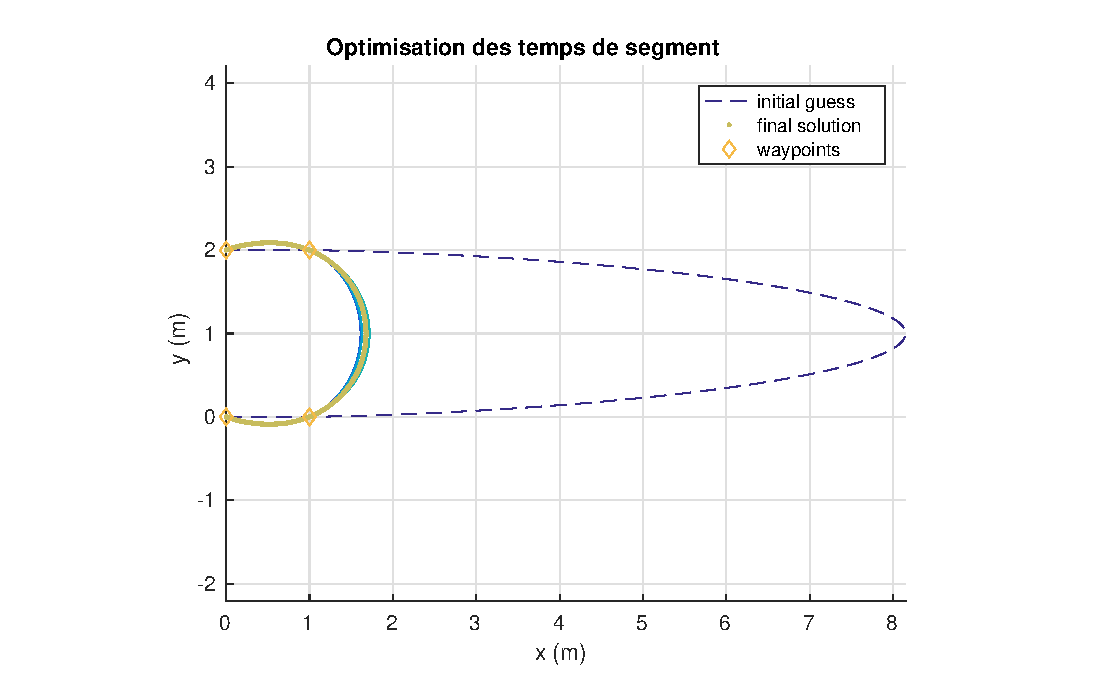
\includegraphics[width=1.2\textwidth]{fig/arc_time_opt}
  \caption{Résultat des itérations, l'allocation de temps initiale donnait beaucoup trop de temps au segment du milieu.}
\end{subfigure}%
\begin{subfigure}{.45\textwidth}
  \centering
  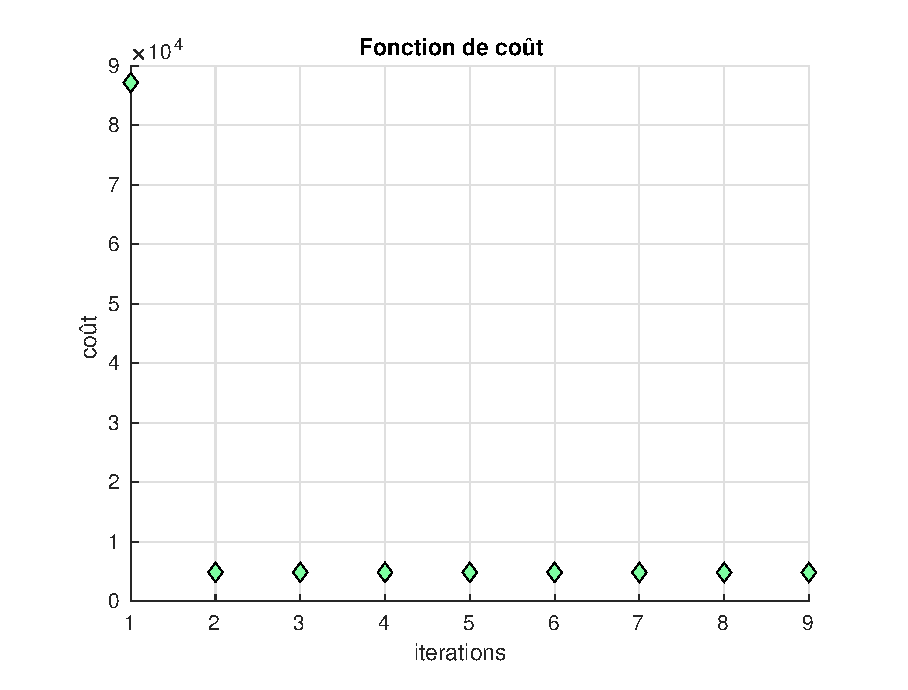
\includegraphics[width=\textwidth]{fig/cost}
  \caption{Valeur de la fonction de coût à chaque itération}
  \label{fig:sub2}
\end{subfigure}
\caption{Comparaison de résultats d'optimisation des temps de segment}
\label{fig:comparaison_opt_temps}
\end{figure}


Dans la figure (\ref{fig:comparaison_opt_temps}) nous voyons le résultat de l'optimisation des segments de temps. Suite à un grand saut d'une ordre de grandeur, le changement à la fonction de coût devient mineur. 
Notre méthode semble s'être approché de la solution en seulement une itération et termine après 7 itérations, le meme nombre que Mellinger. Nous voyons aussi dans le bloc suivant la sortie de console de Matlab lors de l'optimisation.

\begin{verbatim}
>> main_optimt
                                            First-order      Norm of
 Iter F-count            f(x)  Feasibility   optimality         step
    0       1    8.711304e+04    0.000e+00    5.069e+05
    1       3    4.893364e+03    4.166e-12    3.105e+05    1.219e+00
    2       4    4.888882e+03    0.000e+00    3.882e+03    4.061e-03
    3       9    4.879789e+03    4.441e-16    1.242e+03    8.132e-03
    4      13    4.879264e+03    4.441e-16    1.193e+03    4.046e-03
    5      17    4.874708e+03    0.000e+00    1.210e+03    6.915e-02
    6      18    4.860743e+03    0.000e+00    4.416e+01    3.115e-02
    7      19    4.860729e+03    0.000e+00    3.209e+00    5.396e-04

Optimization stopped because the relative changes in all elements of x are
less than options.StepTolerance = 1.000000e-10, and the relative maximum constraint
violation, 0.000000e+00, is less than options.ConstraintTolerance = 1.000000e-06.

Optimization Metric                                           Options
max(abs(delta_x./x)) =   6.25e-11                       StepTolerance =   1e-10 (default)
relative max(constraint violation) =   0.00e+00   ConstraintTolerance =   1e-06 (default)

Elapsed time is 4.171527 seconds.
\end{verbatim}

Nous voyons que le processus prend étonamment longtemps ($4.17$ secondes) quoi que le tout a été calculé sur un vieux laptop avec beaucoup d'applications ouvertes.

\subsection{Implémentation finale en C++}
L'intéret


\subsubsection{Comparaison de solveurs QP}

\subsubsection{Comparaison des solveurs non-linéaires}
\bibliographystyle{abbrv}
\bibliography{bibliography}

\end{document}
